% #######################################
% ########### FILL THESE IN #############
% #######################################
\def\mytitle{ASSIGNMENT-2}
\author{BHAVANI KANIKE}
% #######################################
% #### YOU DON'T NEED TO TOUCH BELOW ####
% #######################################
\documentclass[10pt, a4paper]{article}
\usepackage[a4paper,outer=1.5cm,inner=1.5cm,top=1.75cm,bottom=1.5cm]{geometry}
\twocolumn
\usepackage{graphicx}
\graphicspath{{./images/}}
%colour our links, remove weird boxes
\usepackage[colorlinks,linkcolor={black},citecolor={blue!80!black},urlcolor={blue!80!black}]{hyperref}
%Stop indentation on new paragraphs
\usepackage[parfill]{parskip}
%% Arial-like font
\usepackage{lmodern}
\renewcommand*\familydefault{\sfdefault}
%Napier logo top right
\usepackage{watermark}
%Lorem Ipusm dolor please don't leave any in you final report ;)
\usepackage{karnaugh-map}
\usepackage{tabularx}
\usepackage{lipsum}
\usepackage{xcolor}
\usepackage{listings}
%give us the Capital H that we all know and love
\usepackage{float}
%tone down the line spacing after section titles
\usepackage{titlesec}
%Cool maths printing
\usepackage{amsmath}
%PseudoCode
\usepackage{algorithm2e}

\titlespacing{\subsection}{0pt}{\parskip}{-3pt}
\titlespacing{\subsubsection}{0pt}{\parskip}{-\parskip}
\titlespacing{\paragraph}{0pt}{\parskip}{\parskip}
\newcommand{\figuremacro}[5]{
    \begin{figure}[#1]
        \centering
        \includegraphics[width=#5\columnwidth]{#2}
        \caption[#3]{\textbf{#3}#4}
        \label{fig:#2}
    \end{figure}
}

\lstset{
escapeinside={/*@}{@*/}, language=C++,
basicstyle=\fontsize{8.5}{12}\selectfont,
numbers=left,numbersep=2pt,xleftmargin=2pt,frame=tb,
    columns=fullflexible,showstringspaces=false,tabsize=4,
    keepspaces=true,showtabs=false,showspaces=false,
    backgroundcolor=\color{white}, morekeywords={inline,public,
    class,private,protected,struct},captionpos=t,lineskip=-0.4em,
aboveskip=10pt, extendedchars=true, breaklines=true,
prebreak = \raisebox{0ex}[0ex][0ex]{\ensuremath{\hookleftarrow}},
keywordstyle=\color[rgb]{0,0,1},
commentstyle=\color[rgb]{0.133,0.545,0.133},
stringstyle=\color[rgb]{0.627,0.126,0.941}
}

\thiswatermark{\centering \put(1,-110.0){\includegraphics[scale=0.075]{logo}} }
\title{\mytitle}
%\author{\myauthor\hspace{1em}\\\contact\\\hspace{0.5em}\hspace{0.5em}\mymodule}
\date{}
\hypersetup{pdfauthor=/myauthor,pdftitle=/mytitle,pdfkeywords=/mykeywords}
\sloppy
% #######################################
% ########### START FROM HERE ###########
% #######################################
\begin{document}
\maketitle
\begin{abstract}
 Draw the logic circuit of the following Boolean Expression using only NAND Gates : X.Y + Y.Z
\end{abstract}

\section{Components}

%\begin{table}[]
    \centering
    \begin{tabular}{ |c |c |c |c |}
\hline
\hline
\newline
\newline
\textbf{Components} & \textbf{Value} & \textbf{Quantity} \\
\hline
 %Resistor & 220Ohm & 1 \\ 
 Arduino & UNO & 1 \\  
 %Seven segment Display &  & 1 \\
 %Decoder& 7447&1 \\
 seven segment display& - & 1 \\
 Jumper wires&M-M &18\\
 Breadboard& &1\\
 Resister&150 ohm&1\\
 Decoder&7447&1\\
 \hline
 \end{tabular}
 \vspace{3mm}
 
 %\caption{Table 1.0}
    \label{table1}
%\end{table}

\section{TruthTable}
 This manual shows how to use Arduino with 7447 and sevensegment dispaly to represent pos canonical form for function 'F' in truth table.
   
\begin{tabularx}{0.4\textwidth} { 
  | >{\centering\arraybackslash}X 
  | >{\centering\arraybackslash}X 
  | >{\centering\arraybackslash}X
  | >{\centering\arraybackslash}X | }
\hline
X & Y & Z & F \\
\hline
0 & 0 & 0 & 0\\  
\hline
0 & 0 & 1 & 0 \\ 
\hline
0 & 1 & 0 & 0 \\
\hline
0 & 1 & 1 & 1 \\
\hline
1 & 0 & 0 & 0 \\  
\hline
1 & 0 & 1 & 0 \\ 
\hline
1 & 1 & 0 & 1 \\
\hline
1 & 1 & 1 & 1 \\
\hline
\end{tabularx}

   
\section{HardwareConnections}
\begin{figure}
    \centering
    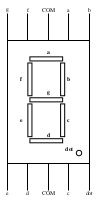
\includegraphics{seven.png}
    \caption{Seven segment display}
    \label{fig:my_label}
\end{figure}
\begin{figure}
    \centering
    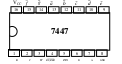
\includegraphics{7447ic.png}
    \caption{Pin diagram of 7447IC}
    \label{fig:my_label}
\end{figure}
\begin{figure}
    \centering
    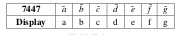
\includegraphics{sevenseg.png}
    \caption{}
    \label{fig:my_label}
\end{figure}
\begin{figure}
    \centering
    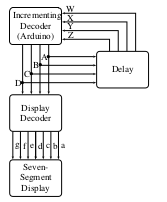
\includegraphics{connect.png}
    \caption{}
    \label{fig:my_label}
\end{figure}

*Make the connections as shown in the Figure3 and Figure4.

*Connect COM pin of seven segment display to Vcc through Resister and Dot pin to ground.

\begin{figure}
    \centering
    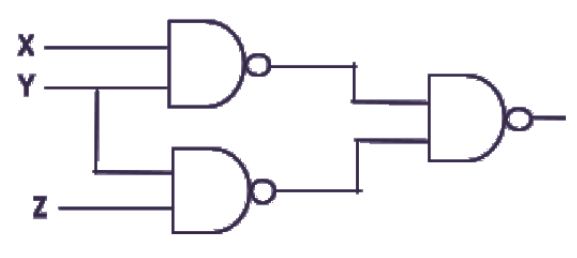
\includegraphics{a1.png}
    \caption{F = XY + YZ}
    \label{fig:my_label}
\end{figure}
\section{Execution}
*Verify the above truth table by using the minimized expression in the following code.

\framebox{
\url{https://github.com/bhavani360/FWC_assignments}}
\bibliographystyle{ieeetr}
\end{document}